% !TEX root =  ../report.tex
\begin{figure*}[ht!]
    \centering
    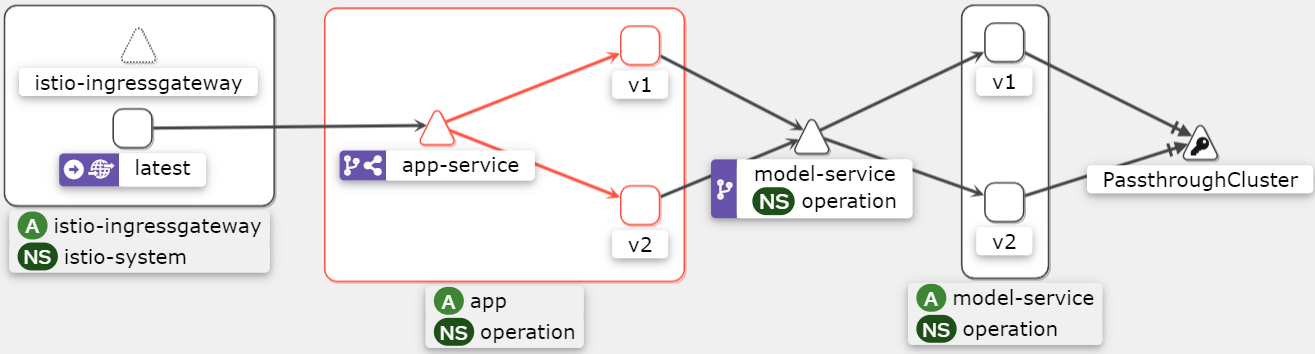
\includegraphics[width=18cm]{report/images/kiali.png}
    \caption{Deployment of operation}
    \label{fig:kiali}
\end{figure*}
\begin{figure*}[!ht]
    \centering
    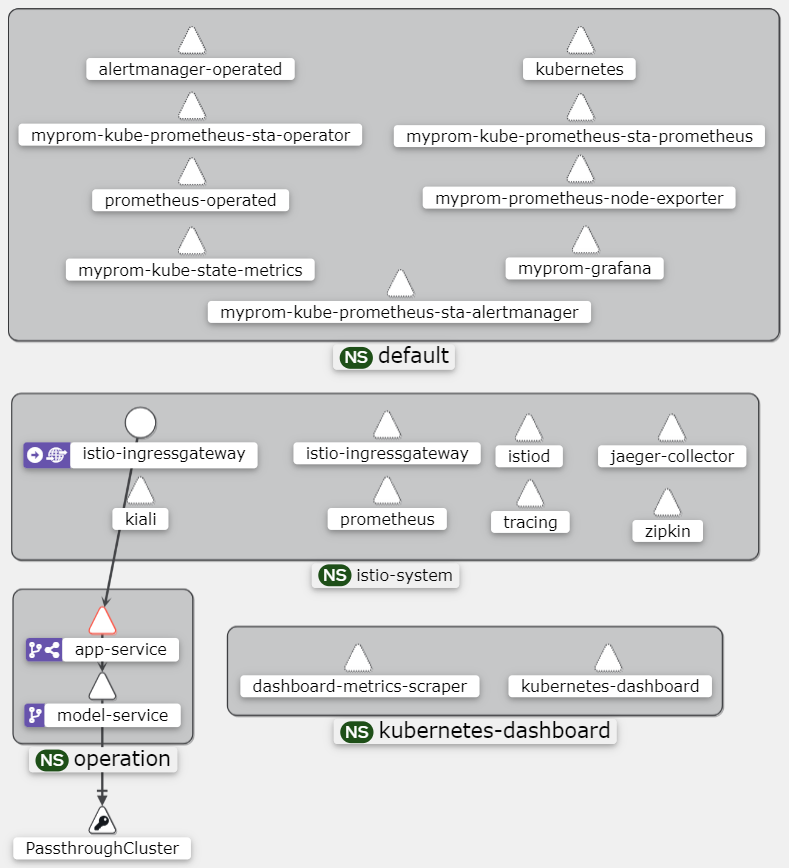
\includegraphics[width=13cm]{report/images/kialiServices.png}
    \caption{Entire deployment cluster}
    \label{fig:kialiall}
\end{figure*}
\clearpage
\section{Deployment Documentation}
This section covers the deployment and data flow of the project. The project is deployed on a minikube cluster, this allows for scaling of the project as well as stability through backup deployment replicas.

\subsection{Deployment structure}
The deployment structure is visualized in \autoref{fig:kiali}. It consists of two main services with each having two deployment versions for a potential canary release:

\begin{enumerate}
    \item \textbf{app-service}: App-service handles the front-end of the application and serves the page that the user directly interacts with. This is done through two flask deployments each running a different version. Each of these deployments consist of only 1 replica and therefore do not provide redundancy out of the box. This can be scaled up to improve availability.
    \item \textbf{model-service}: Model-service handles the back-end of the application and provides the "predict" endpoint for the app to interact with, which returns the prediction result given an url. This is done through two flask deployments hosting the model each running a different version. Each of these deployments also consist of only 1 replica.
\end{enumerate}


\subsection{Data flow}
The Ingress gateway is provided by Istio and serves as the entry point to the application. The request is then handled by the app-service which forwards the request to one of the two deployment versions with equal probability (50/50). The user is then able to make a prediction on the app. The app then sends a post request to the model-service which forwards it to the corresponding model-service deployment version. The prediction is then directly returned through the passthrough cluster.

\subsection{Full cluster deployment}
The project furthermore employs various monitoring tools on the cluster, these include Prometheus and Grafana. Additionally various other dashboards can be added to the cluster such as the Minikube, Jaeger and Kiali dashboard. The full deployment of all clusters can be found in \autoref{fig:kialiall}. Prometheus scrapes the "/metrics" endpoint of the model-service deployments to keep track of various metrics. Grafana can then be connected to prometheus to provide a intuitive dashboard of the various metrics.


